\documentclass{article}
\usepackage{graphicx}
\usepackage{amsmath}
\usepackage{amssymb}
\usepackage{enumitem}
\usepackage{hyperref}

\begin{document}
\title{Lista de Exercícios 1 - Cálculo 2}
\author{Débora D'Angelo Reina de Araujo}
\date{\today}

\maketitle

\begin{enumerate}
    \item Resolver exercícios do 1 ao 11 do Apostol manualmente e usando CAS. \\
    Compute the derivatives $F'(t)$ and $F''(t)$ for each of the vector-valued functions in Exercises 1 through 6. \
        \begin{enumerate}[label=1.\arabic*.]
            \item $F(t) = (t, t^2, t^3, t^4)$ \\
                \\
                $F'(t) = (1, 2t, 3t^2, 4t^3)$ \\
                $F''(t) = (0, 2, 6t, 12t^2)$ \\
            \item $F(t) = (cos(t), sin^2(t), sin(2t), tan(t))$ \\
                \\
                Vamos resolver por partes $F'(t)$: \
                \begin{itemize}
                    \item $(cos(t))' = -sin(t)$ \
                    \item $(sin^2(t))'= 2sin(t) \cdot cos(t)$ \
                    \item $(sin(2t))' = 2cos(2t)$ \
                    \item $(tan(t))' = (sin(t) \cdot \frac{1}{cos(t)})' = cos(t) \cdot \frac{1}{cos(t)} + sin(t) \cdot (cos^{-1}(t)) = \frac{cos(t)}{cos(t)} + sin(t) \cdot (-1)(cos^{-2}(t))(-sin(t)) = \frac{cos^2(t)}{cos^2(t)} + \frac{sin^2(t)}{cos^2(t)} = \frac{1}{cos^2(t)} = sec^2(t) $ \
                \end{itemize} \
                Agora, iremos por partes $F''(t)$: \
                \begin{itemize}
                    \item $(cos(t))'' = (-sin(t))' = -cos(t)$ \
                    \item $(sin^2(t))''= (2sin(t) \cdot cos(t))' = (2sin(t))'(cos(t)) + 2sin(t)(cos(t))' = 2cos^2(t) - 2sin^2(t) $ \
                    \item $(sin(2t))'' = (2cos(2t))' = 2(cos(2t))' = 2(-sin(2t)2) = -4sin(2t)$ \
                    \item $(tan(t))'' = (sec^2(t))' = (cos^{-2}(t))' = -2cos^{-3}(t)(-sin(t)) = \frac{2sin(t)}{cos^3(t)} = 2tan(t)(sec^2(t))$ \
                \end{itemize} \
                Portanto: \\
                $F'(t) = (-sin(t), 2sin(t) \cdot cos(t), 2cos(2t), sec^2(t))$ \\
                $F''(t) = (-cos(t), 2cos^2(t) - 2sin^2(t), 2(-sin(2t)2) = -4sin(2t),  2tan(t)(sec^2(t)))$ \\
            \item $F(t) = (arcsin(t), arccos(t))$ \\
                \\
                $F'(t) = (\frac{1}{\sqrt{1-x^2}}, \frac{-1}{\sqrt{1-x^2}})$ \\
                $F''(t) = (\frac{x}{(1-x^2)^{\frac{3}{2}}}, \frac{-x}{(1-x^2)^{\frac{3}{2}}})$ \\
            \item $F(t) = 2e^t\textbf{i} + 3e^t\textbf{j}$ \\
                \\
                $F'(t) = 2e^t\textbf{i} + 3e^t\textbf{j}$ \\
                $F''(t) = 2e^t\textbf{i} + 3e^t\textbf{j}$\\
            \item $F(t) = cosh(t) \textbf{i} + sinh(2t) \textbf{j} + e^{-3t}\textbf{k}$ \\
                \\
                $F'(t) = sinh(t) \textbf{i} + 2cosh(2t) \textbf{j} + -3e^{-3t} \textbf{k}$ \\ 
                $F''(t) = cosh(t) \textbf{i} + 4sinh(2t) \textbf{j} + 9e^{-3t} \textbf{k} $ \\
            \item $F(t) = log(1+t^2)\textbf{i} + arctan(t) \textbf{j} + \frac{1}{1+t^2}\textbf{k}$ \\
                \\
                $F'(t) = \frac{2t}{1+t^2}\textbf{i} + \frac{1}{1+t^2}\textbf{j} - \frac{2t}{(1+t^2)^2}\textbf{k} $ \\
                Agora, por partes: \
                \begin{itemize}
                    \item $(\frac{2t}{1+t^2})' = (2t)'(1+t^2)^{-1} + 2t((1+t^2)^{-1})' = (2t)'(1+t^2)^{-1} + 2t(-1)(1+t^2)^{-2}(1+t^2)' = \frac{2}{1+t^2} - \frac{-4t^2}{(1+t^2)^2} $ \
                    \item $(\frac{1}{1+t^2})' = \frac{-2t}{(1+t^2)^2}$ \
                    \item $(\frac{2t}{(1+t^2)^2})' = \frac{2}{(1+t^2)^2} + \frac{2t(-2)(2t)}{(1+t^2)^{3}} = \frac{2}{(1+t^2)^2} - \frac{8t^2}{(1+t^2)^3}$ \
                \end{itemize} \
                $F''(t) = (\frac{2}{1+t^2} - \frac{-4t^2}{(1+t^2)^2})\textbf{i} + \frac{-2t}{(1+t^2)^2} \textbf{j} + (\frac{2}{(1+t^2)^2} - \frac{8t^2}{(1+t^2)^3}) \textbf{k}$ \\
            \item (\textbf{Importante!}) Let F be the vector-valued function given by \\
                $$F(t) = \frac{2t}{1+t^2}\textbf{i} + \frac{1-t^2}{1+t^2}\textbf{j} + \textbf{k}$$. \
                Prove that the angle between $F(t)$ and $F'(t)$ is constant, that is, independent of t. \\
                \\
                $F'(t)=((2t)(1+t^2)^{-1})' \textbf{i} + ((1-t^2)(1+t^2)^{-1})' \textbf{j} + (1)' \textbf{k}$ \\
                $F'(t)=(2(i+t^2)^{-1} + (2t)(-1)(1+t^2)^{-2}(2t)) \textbf{i} + ((-2t)(1+t^2)^{-1} + (1-t^2)(-1)(1+t^2)^{-2}(2t)) \textbf{j} + 0 \textbf{k}$ \\
                $F'(t)=(\frac{2}{1+t^2} - \frac{4t^2}{(1+t^2)^2}) \textbf{i} + (\frac{-2t}{1+t^2} + \frac{-2t(1-t^2)}{(1+t^2)^2}) \textbf{j} + 0 \textbf{k}$ \\
                $F'(t)=(\frac{2(1+t^2) - 4t^2}{(1+t^2)^2}) \textbf{i} - (\frac{2t(1+t^2) + 2t(1-t^2)}{(1+t^2)^2}) \textbf{j} + 0 \textbf{k}$ \\
                $F'(t)=(2\frac{1+t^2 - 2t^2}{(1+t^2)^2}) \textbf{i} - (\frac{2t+2t^3 + 2t-2t^3)}{(1+t^2)^2}) \textbf{j} + 0 \textbf{k}$ \\
                $F'(t)=(2\frac{1-t^2}{(1+t^2)^2}) \textbf{i} - (\frac{4t}{(1+t^2)^2}) \textbf{j} + 0 \textbf{k}$ \\
                \\
                Agora vamos calcular o produto escalar $F(t) \cdot F'(t)$: \\
                $F(t) \cdot F'(t) = (\frac{2t}{1+t^2})(2\frac{1-t^2}{(1+t^2)^2}) + (\frac{1-t^2}{1+t^2})(\frac{-4t}{(1+t^2)^2}) + (1)(0)$ \\
                $F(t) \cdot F'(t) = \frac{4t(1-t^2)}{(1+t^2)^3} - \frac{4t(1-t^2)}{(1+t^2)^3} + 0$ \\
                $F(t) \cdot F'(t) = 0$ \\
                \\
                Logo $F(t)$ e $F'(t)$ são perpendiculares, ou seja, o ângulo entre eles é constante. \\
                \\
            Compute the vector-valued integrals in Exercises 8 through 11. \
            \item $\int_{0}^{1} (t, \sqrt{t}, e^t)dt$ \\
                \\
                 $\int_{0}^{1} (t, \sqrt{t}, e^t)dt = (\frac{t^2}{2}|_{0}^{1}, \frac{2}{3}t^{\frac{3}{2}}|_{0}^{1}, e^t|_{0}^{1}) + C$ \\
                 $\int_{0}^{1} (t, \sqrt{t}, e^t)dt = (\frac{1}{2}, \frac{2}{3}, e - 1) + C$ \\
            \item $\int_{0}^{\frac{\pi}{4}} (sin(t), cos(t), tan(t))dt$ \
                \\
                $\int_{0}^{\frac{\pi}{4}} (sin(t), cos(t), tan(t))dt = (-cos(t)|_{0}^{\frac{\pi}{4}}, sin(t)|_{0}^{\frac{\pi}{4}}, log(sec(t))|_{0}^{\frac{\pi}{4}}) + C$ \\
                $\int_{0}^{\frac{\pi}{4}} (sin(t), cos(t), tan(t))dt = (\frac{2-\sqrt{2}}{2}, \frac{\sqrt{2}}{2}, \frac{log(2)}{2}) + C$ \\
            \item $\int_{0}^{1} (\frac{e^t}{1+e^t}\textbf{i} + \frac{1}{1+e^t}\textbf{j})dt$ \
                \\
                $\int_{0}^{1} (\frac{e^t}{1+e^t}\textbf{i} + \frac{1}{1+e^t}\textbf{j})dt = log(e^t+1)\textbf{i}|_{0}^{1} + (t-log(e^t+1))\textbf{j}|_{0}^{1} + C$\\
                $\int_{0}^{1} (\frac{e^t}{1+e^t}\textbf{i} + \frac{1}{1+e^t}\textbf{j})dt = (log(e+1) - log(2))\textbf{i} + (1 - log(e+1) + log(2))\textbf{j} + C$\\
            \item $\int_{0}^{1} (te^t\textbf{i} + t^2e^t\textbf{j} + te^{-t}\textbf{k})dt$ \\
                $\int_{0}^{1} (te^t\textbf{i} + t^2e^t\textbf{j} + te^{-t}\textbf{k})dt = ((t-1)e^t)\textbf{i}|_{0}^{1} + ((t^2-2t+2)e^t)\textbf{j}|_{0}^{1} - ((t+1)e^{-1})\textbf{k}|_{0}^{1} + C$\\
                $\int_{0}^{1} (te^t\textbf{i} + t^2e^t\textbf{j} + te^{-t}\textbf{k})dt = 1\textbf{i} + (e - 2)\textbf{j} + (-2e^{-1} + 1)\textbf{k} + C$ \\
        \end{enumerate}
    \item (\textbf{Importante!}) Encontrar uma curva parametrizada $\alpha(t) : t \in I \to \mathbb{R}^2$; cujo traço seja o círculo $x^2 + y^2 = 1$; de maneira que t percorra o círculo no sentido anti-horário e tenhamos $\alpha(0) = (0, 1)$. Faça o desenho em um sistema CAS, incluindo a animação do vetor tangente percorrendo a curva. \\    
        \begin{figure}[!h]
            \centering
            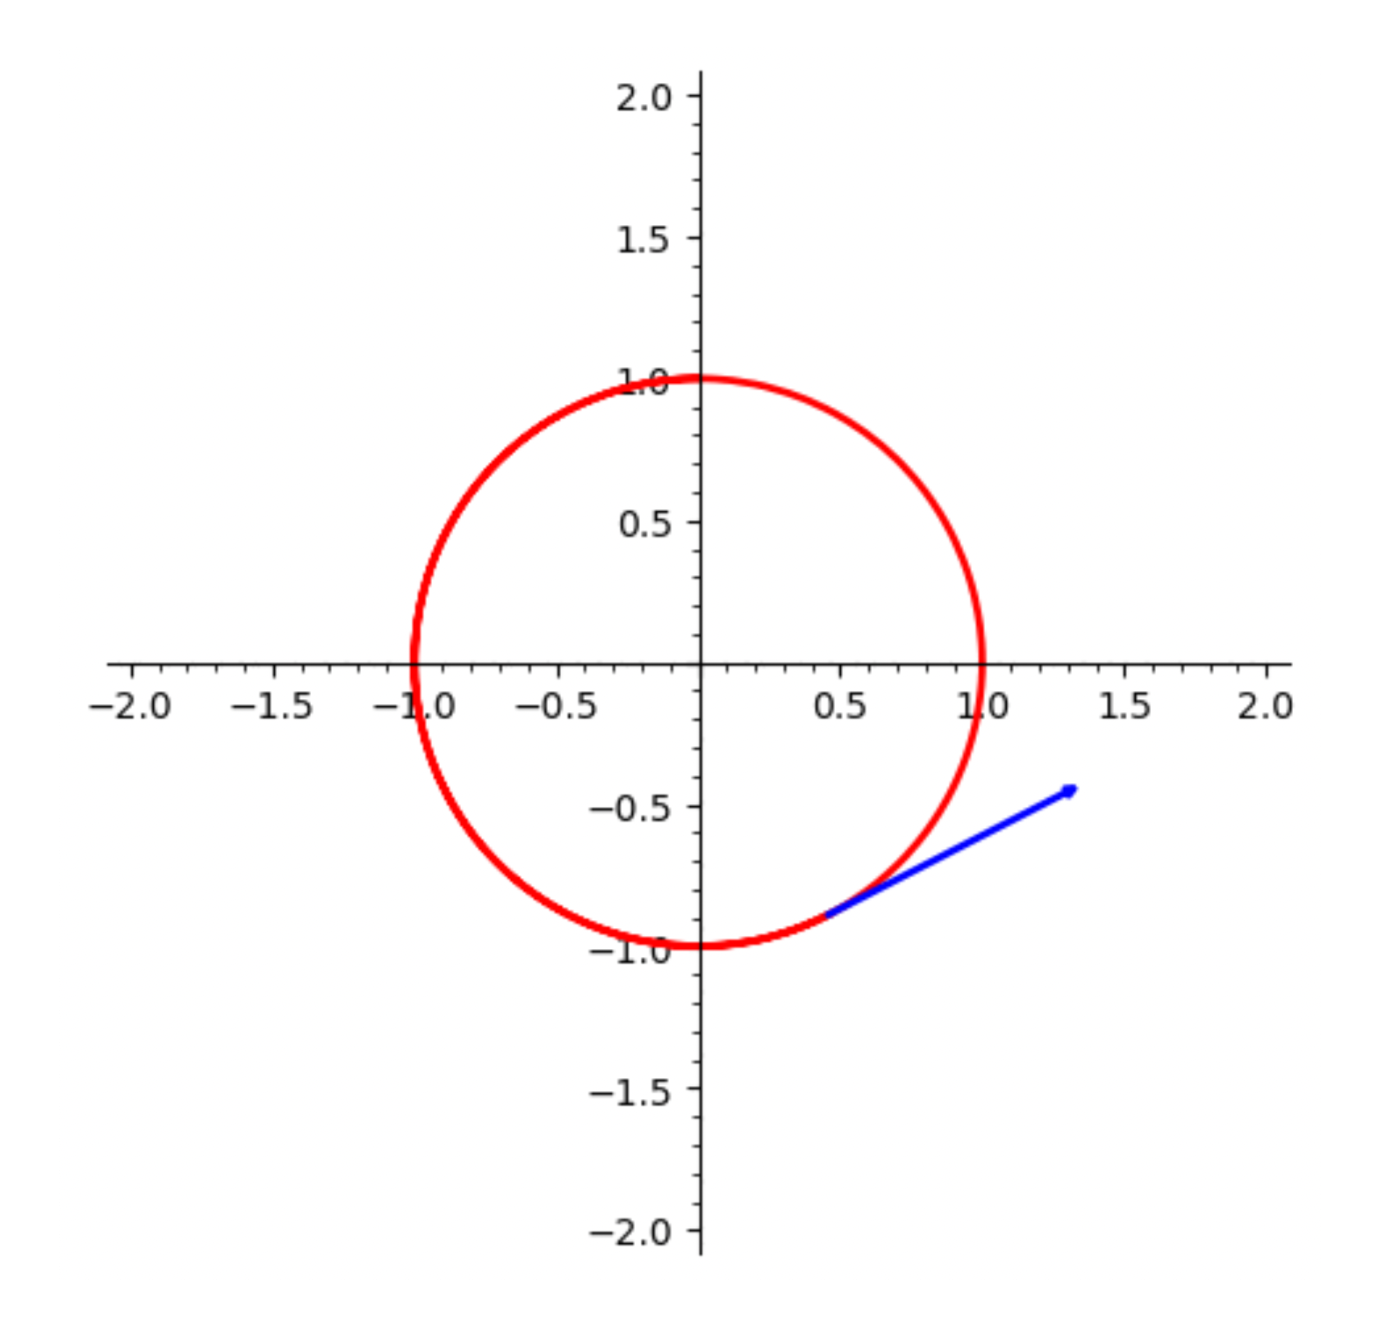
\includegraphics[width=0.35\textwidth]{imgs/curva_vector.png}
            \label{fig:exercício 2}
        \end{figure}
        \\ $\alpha(t) = (-sin(t), cos(t))$
    \item (\textbf{Importante!}) A \textit{limaçon} (ou caracol de Pascal) é a curva parametrizada \
        $$\gamma(t) = ((1+2cos(t)) \cdot cos(t); (1+2cos(t)) \cdot sin(t)); t \in \mathbb{R}$$
        Faça o desenho desta curva em um sistema CAS. Observe que o ponto (0, 0) pertence ao traço da curva, e ache o vetor tangente nesse ponto. \
        \begin{figure}[!h]
            \centering
            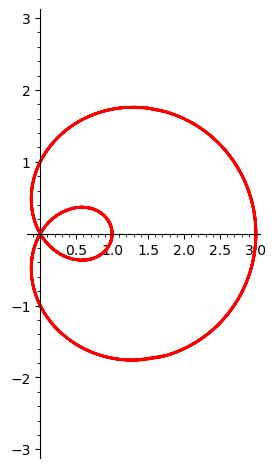
\includegraphics[width=0.35\textwidth]{imgs/limacon.png}
            \label{fig:exercício 3}
        \end{figure}
        \\ Perceba que $\gamma(\frac{2\pi}{3}) = ((1+2cos(\frac{2\pi}{3})) \cdot cos(\frac{2\pi}{3}); (1+2cos(\frac{2\pi}{3})) \cdot sin(\frac{2\pi}{3})) $\\
        $\gamma(\frac{2\pi}{3}) = ((1+2*\frac{-1}{2})\cdot\frac{-1}{2}, (1+2*\frac{-1}{2})\cdot\frac{\sqrt{3}}{2}) = (0, 0) $ \\
    \item A \textit{Cissoide de Diocles} é a curva definida implicitamente pela equação \
        $$x^3+xy^2-2ay^2=0$$ \
        Encontre uma parametrização para esta curva. Faça o desenho em um sistema CAS, incluindo a animação do vetor tangente percorrendo a curva. Busque informação para entender qual o fenomeno modelado por esta curva que a tornou famosa. (Dica: use $y = xt$ para encontrar uma a parametrização da curva.) \\
        \\
        Usando $y = xt$, temos:
            $$ x^3 + x^3t^2 - 2ax^2t^2 = 0 $$
            para $x \neq 0, temos:$
            $$ \frac{x^3 + x^3t^2 - 2ax^2t^2}{x^2} = \frac{0}{x^2} $$
            $$ x = \frac{2at^2}{1+t^2} $$
            $$ y = \frac{2at^3}{1+t^2} $$
            Então temos:
            $$\gamma(t) = (\frac{2at^2}{1+t^2}, \frac{2at^3}{1+t^2})$$
            \begin{figure}[!h]
                \centering
                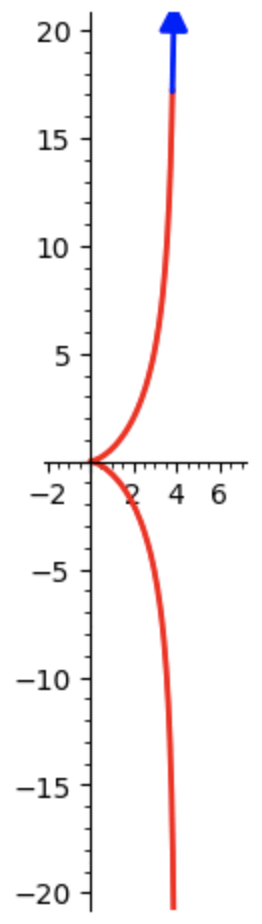
\includegraphics[width=0.35\textwidth]{imgs/cissoide_de_diocles.png}
                \label{fig:exercício 4}
            \end{figure} 
            Observe a imagem da curva com $a = 2$.
    \item o \textit{Folium de Descartes} é definido implicitamente pela equação \
        $$x^3+y^3 = 3xy$$ \
        Encontre uma parametrização para esta curva. Faça o desenho em um sistema CAS, incluindo a animação do vetor tangente percorrendo a curva. A descrição implicita desta curva da origem a uma familia de curvas da forma \
        $$F_{\epsilon}(x, y) = x^3 + y^3 - 3xy - \epsilon$$ \
        \\
        Usando $y = xt$, temos:
        $$x^3+xˆ3t^3-3x^2t = 0$$
        para $x \neq 0$, temos:
        $$\frac{x^3+x^3t^3-3x^2t}{x^2} = \frac{0}{x^2}$$
        $$x = \frac{3t}{1+t^3}$$
        $$y = \frac{3t^2}{1+t^3}$$
        Então temos:
        $$\gamma(t) = (\frac{3t}{1+t^3}, \frac{3t^2}{1+t^3})$$
        \begin{figure}[!h]
            \centering
            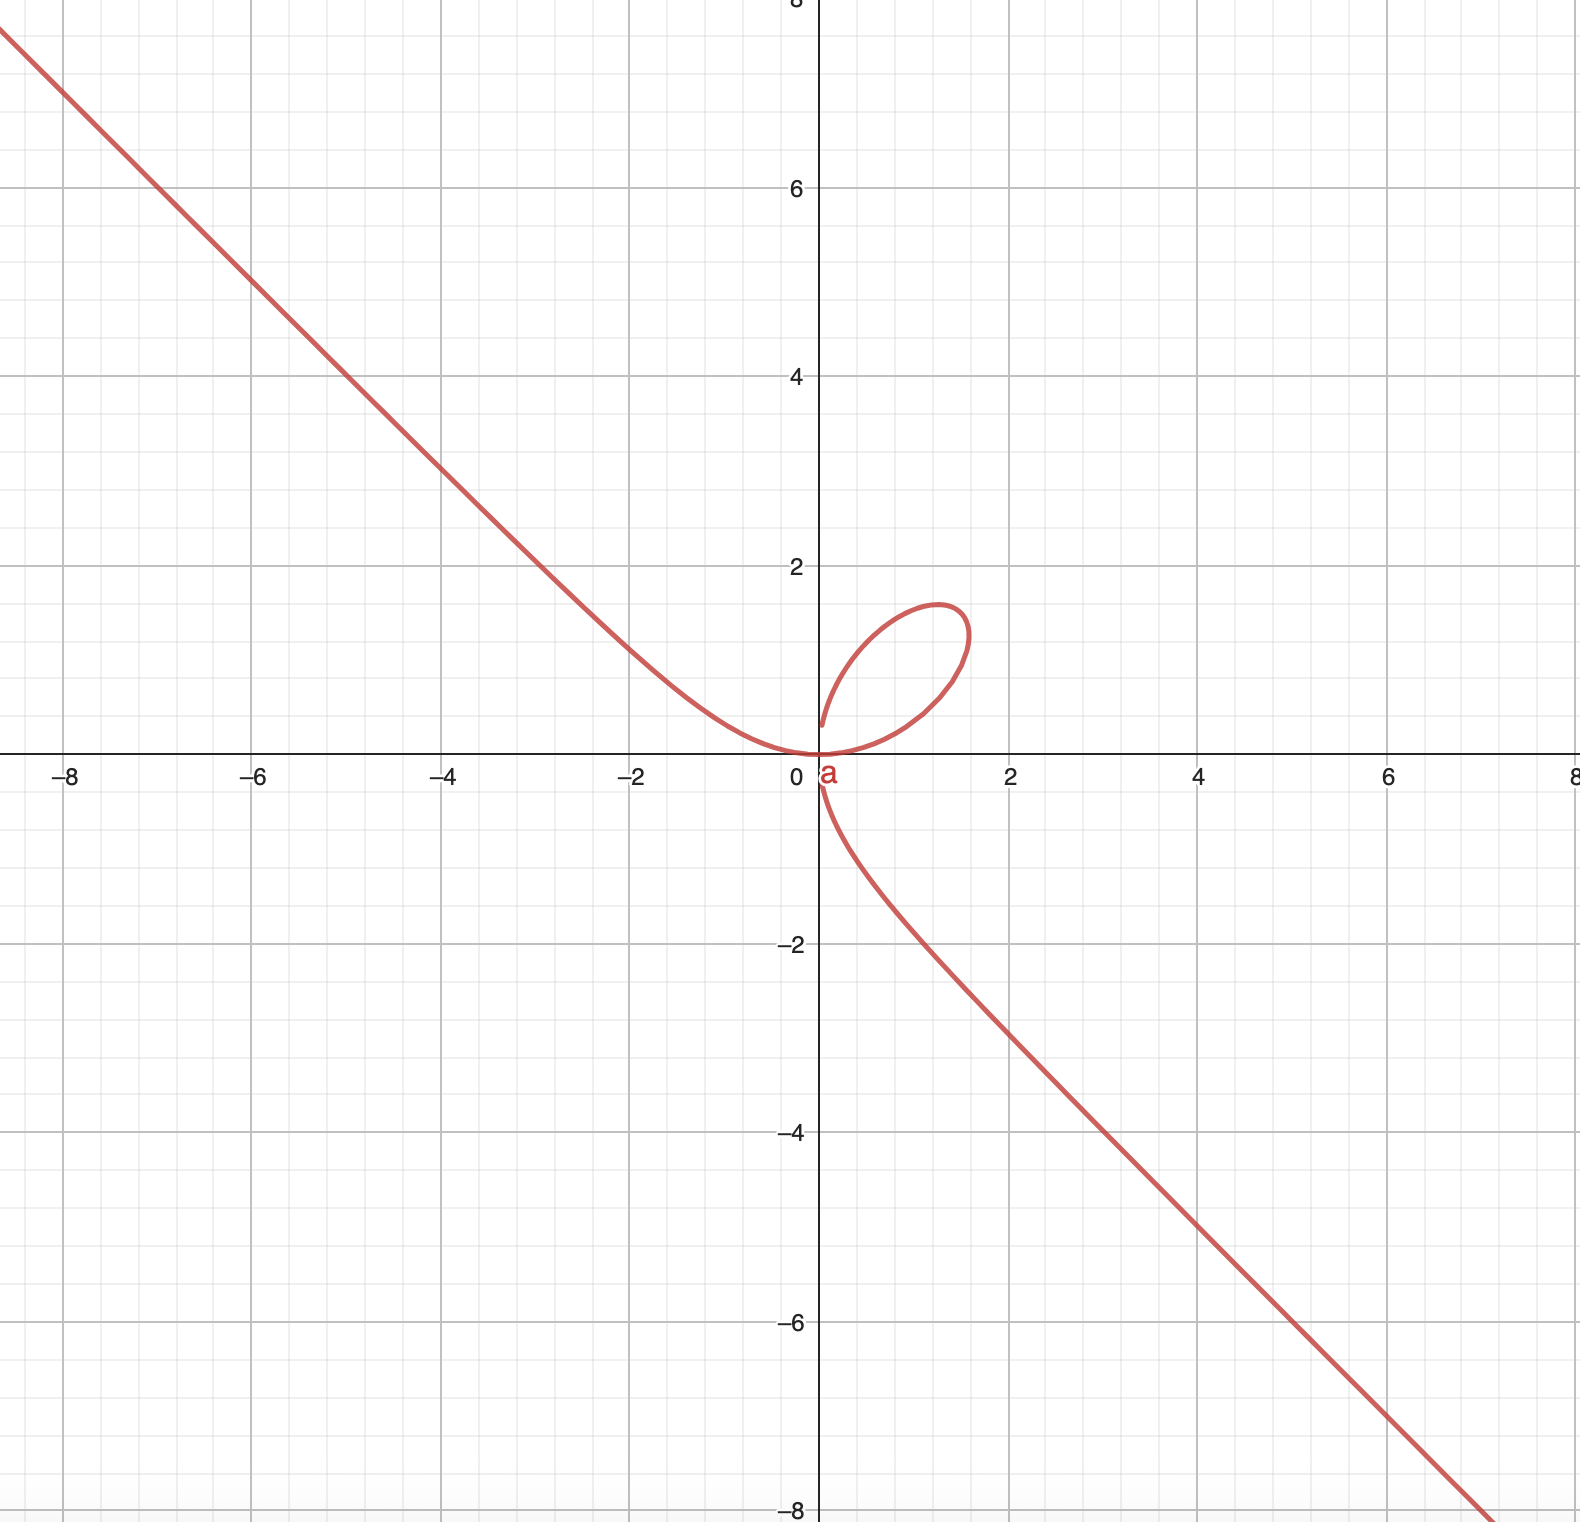
\includegraphics[width=0.35\textwidth]{imgs/folium_de_descartes.png}
            \label{fig:exercício 5}
        \end{figure}
    \item Desenhe as seguintes parametrizações da parábola $\alpha(t) = (t,t^2)$ e $\gamma(t) = (t^3,t^6)$ em ambiente computacional, utilizando sistemas de computação simbólica. Inclua a animação do vetor tangente percorrendo a curva. Mostre que $\alpha$ é curva regular e $\gamma$ não é regular. (\textbf{Desafio:}) Qual seria a função naturalmente candidata a ser uma reparametrização entre as duas parametrizações? Porque falha? \
        \begin{figure}[!h]
            \centering
            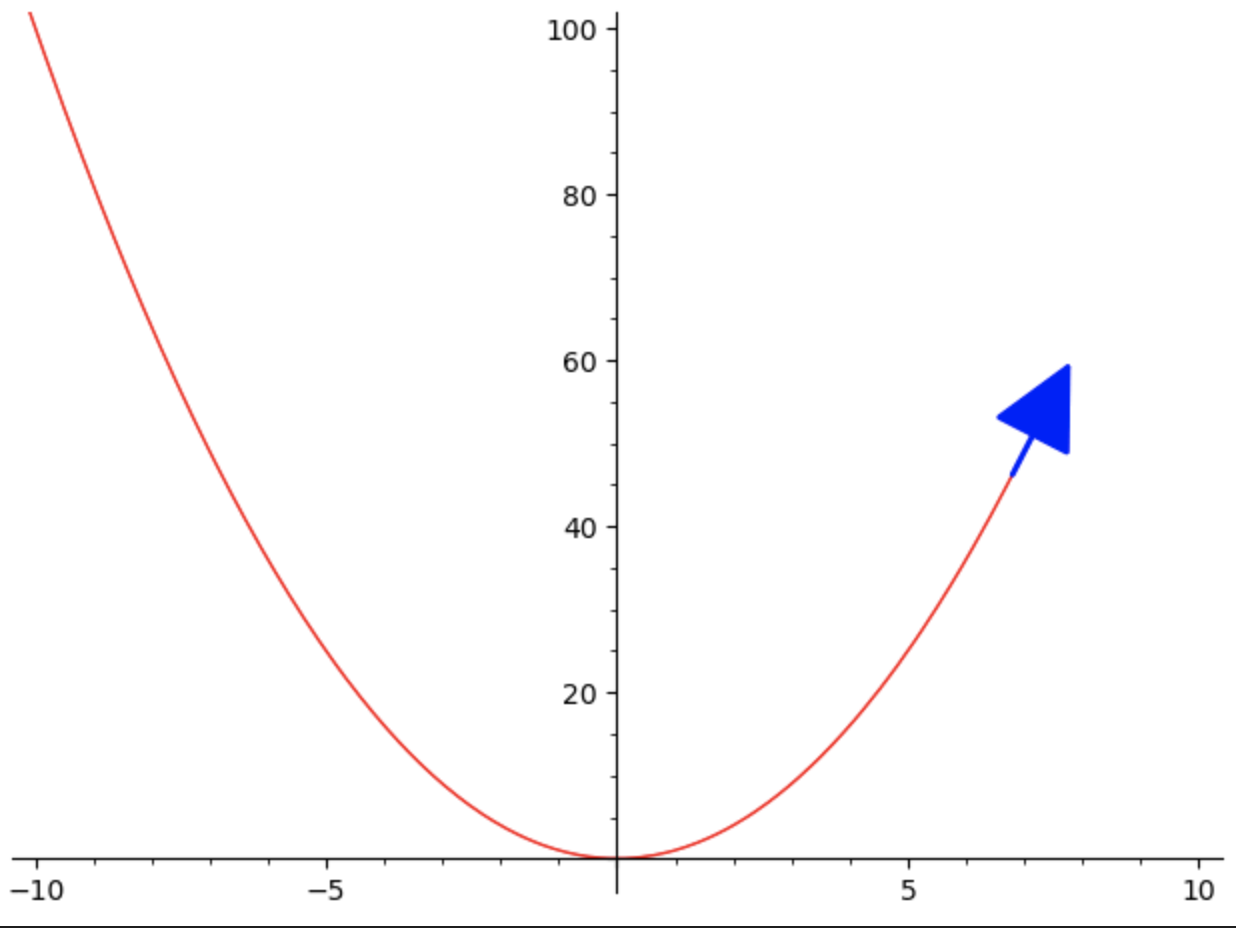
\includegraphics[width=0.35\textwidth]{imgs/curva2.png}
            \label{fig:exercício 6.1}
            \caption{Curva $\alpha$}
        \end{figure}
        \begin{figure}[!h]
            \centering
            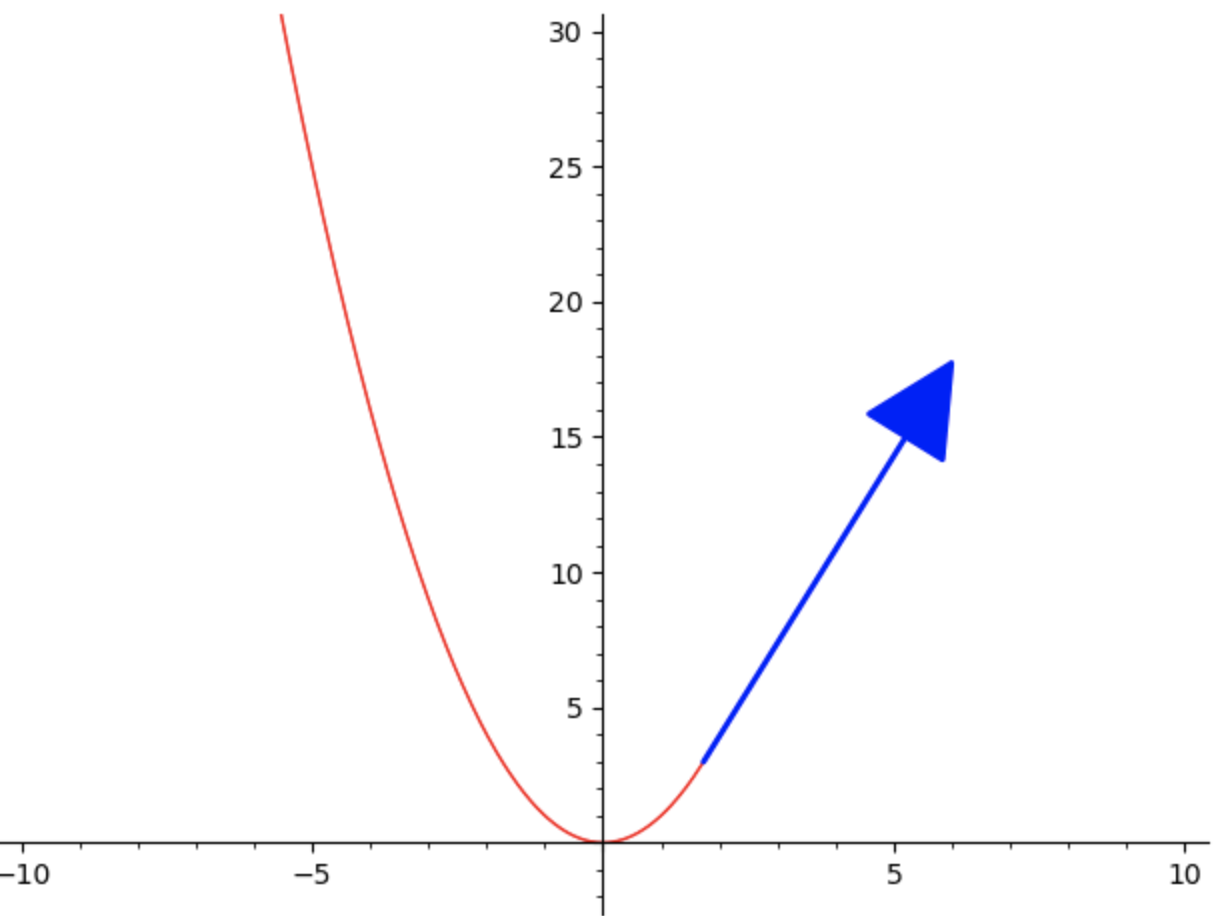
\includegraphics[width=0.35\textwidth]{imgs/curva3.png}
            \label{fig:exercício 6.2}
            \caption{Curva $\gamma$}
        \end{figure}
        \\
        \\
        $\alpha'(t) = (1, 2t)$, logo $\alpha'(t) \neq 0$ para qualquer valor de $t$, portanto $\alpha$ é regular. \\
        $\gamma'(t) = (3t^2, 6t^5)$, logo $\gamma'(t=0) = 0$, ou seja, não é regular. \\
    \item (\textbf{Importante!}) Escolha uma curva "famosa" de sua preferência, desenhe uma animação da curva e seus vetores tangentes para uma dada parametrização e discuta a conveniência de uma nova parametrização ao avaliar a maneira como a trajetória está sendo percorrida. Referência na web de curvas famosas: \href{https://mathshistory.st-andrews.ac.uk/
    Curves/}{\textbf{https://mathshistory.st-andrews.ac.uk/Curves/}} \
        \\
        A curva escolhida foi a Leminiscata de Bernouli. 
        \begin{figure}[!h]
            \centering
            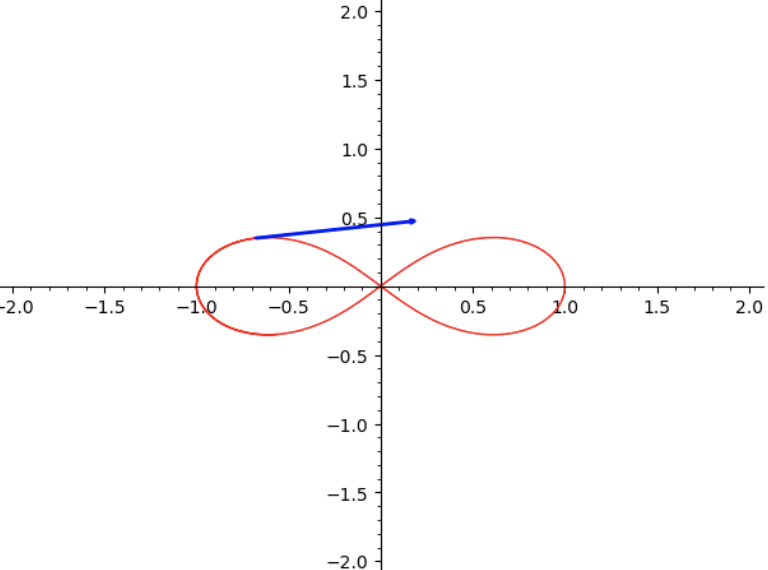
\includegraphics[width=0.35\textwidth]{imgs/leminiscata.png}
            \label{fig:exercício 7}
        \end{figure}
        \\
        Podemos reparametrizar caso quisessemos que a imagem fosse traçada no sentido oposto, ou caso quisessemos que a velocidade fosse normalizada ou que o traço começasse de algum outro ponto, como é o caso do exercício 2.
    \item Obtenha uma curva regular $\alpha : \mathbb{R} \to \mathbb{R}^2$ tal que $\alpha(0) = (2, 0)$ e $\alpha'(t) = (t^2, e^t)$. \
        \\
        $\alpha(t) = (\frac{t^3}{3}, e^t) + C$ \\
        Para que $\alpha(0) = (2, 0)$, temos que $C = (2, -1)$, logo: \\
        $\alpha(t) = (\frac{t^3}{3} + 2, e^t - 1)$ \\
        E $\alpha$ é regular, pois $e^t \neq 0$ para todo $t \in \mathbb{R}$. \
    \item (\textbf{Importante!}) Seja $\alpha : I \to \mathbb{R}^2$ uma curva regular. Prove que $||\alpha'(t)||$ é constante se, e somente se, para cada $t \in I$, o vetor $\alpha''(t)$ é ortogonal a $\alpha'(t)$. \\
        \\
        Partindo de $||\alpha'(t)|| = c$, onde $c$ é uma constante, sabemos que $||\alpha'(t)||^2 = c^2$, ou seja, $||\alpha'(t)||^2$ também é constante. \\
        Vamos chamar $g(t) = ||\alpha'(t)||^2 = \alpha'(t) \cdot \alpha'(t) = c^2$ \\
        Logo $g'(t) = 0$, portanto: \\
        $g'(t) = \alpha''(t)\alpha'(t) + \alpha'(t)\alpha''(t) = 2\alpha'(t)\alpha''(t) = 0$ \\
        Portanto $\alpha''(t)$ é ortogonal a $\alpha'(t)$. \\
        \\
        Agora, partindo de $\alpha''(t)$ ortogonal a $\alpha'(t)$, temos que: \\
        $g'(t) = \alpha''(t)\alpha'(t) + \alpha'(t)\alpha''(t) = 2\alpha'(t)\alpha''(t) = 0$ \\
        Logo:\\
        $g(t) = \int g'(t) = 0 + C$ \\
        $g(t) = ||\alpha'(t)||^2 = C \Rightarrow ||\alpha'(t)|| = \sqrt{C}$
        Portanto $||\alpha'(t)||$ é constante. \\

    \item Considere a espiral logaritmica $\gamma : \mathbb{R} \to \mathbb{R}^2$ definida por $\gamma(t) = (e^t \cdot cos(t), e^t \cdot sin(t))$. Desenhe a curva em ambiente computacional e mostre o ângulo entre $\gamma(t)$ e o vetor tangente em $\gamma(t)$ não depende de t. \ 
        \\
        Considere
        $$cos(\theta) = \frac{\gamma(t) \cdot \gamma'(t)}{||\gamma(t)|| \cdot ||\gamma'(t)||}$$
        $$||\gamma(t)||^2 = (e^t \cdot cos(t))^2 + (e^t \cdot sin(t))^2 = e^{2t} (cos^2(t) + sin^2(t)) = e^{2t} \Rightarrow ||\gamma(t)|| = e^t $$
        $$\gamma'(t) = (e^tcos(t)-e^tsin(t), e^tsin(t)+e^tcos(t))$$
        $$||\gamma'(t)||^2 = (e^t \cdot cos(t) - e^t \cdot sin(t))^2 + (e^t \cdot sin(t) + e^t \cdot cos(t))^2 = 2e^{2t} \Rightarrow ||\gamma'(t)|| = e^t\sqrt{2} $$
        $$\gamma(t) \cdot \gamma'(t) = e^{2t}(cos^2(t) - cos(t)sin(t)+cos(t)sin(t) + sin^2(t)) = e^{2t}$$
        Portanto:
        $$cos(\theta) = \frac{e^{2t}}{e^t \cdot e^2\sqrt{2}} = \frac{1}{\sqrt{2}} \Rightarrow \theta = \frac{pi}{4}$$
        Logo o angulo entre $\gamma(t)$ e $\gamma'(t)$ é constante e igual a 45$^o$. \\
        \begin{figure}[!h]
            \centering
            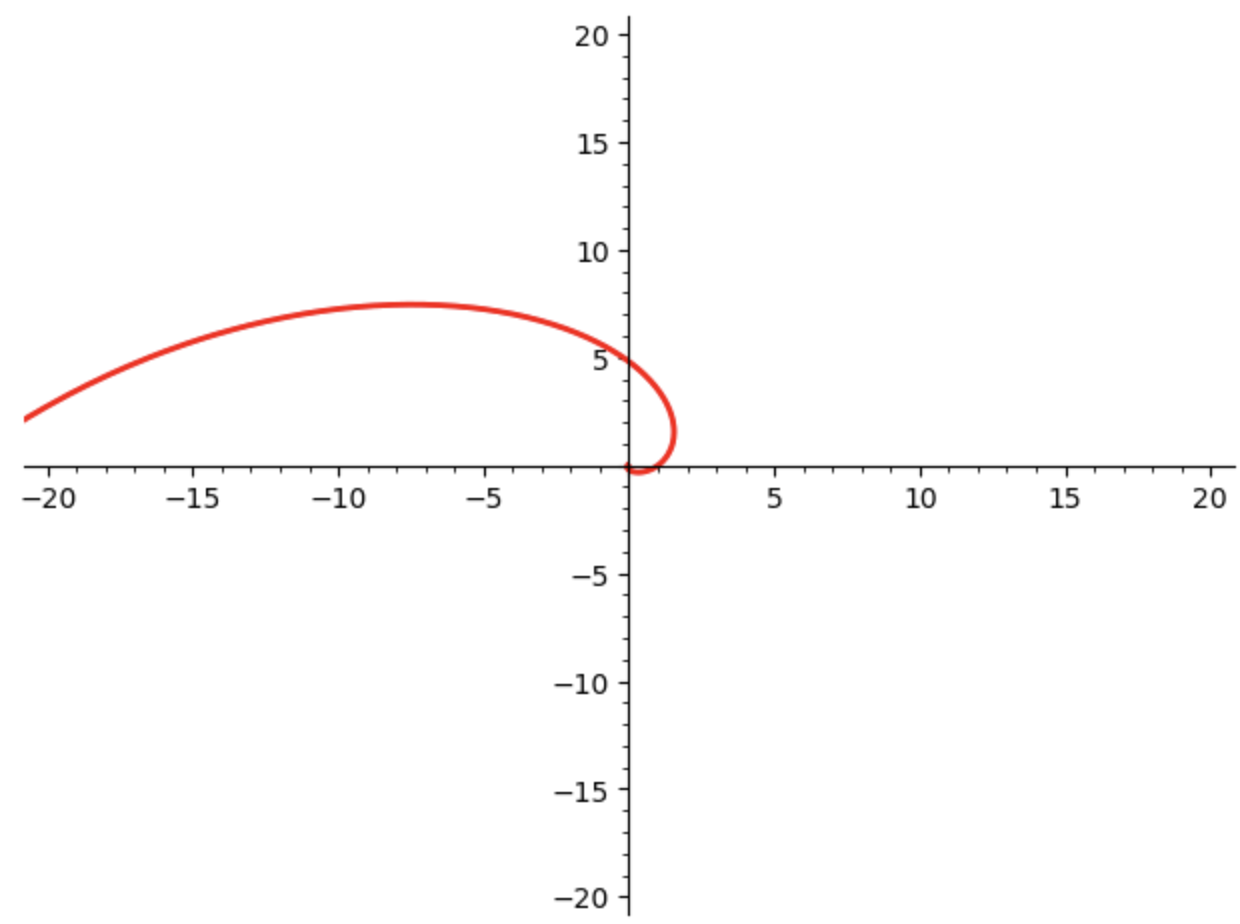
\includegraphics[width=0.2\textwidth]{imgs/esp_log.png}
            \label{fig:exercício 7}
        \end{figure}
\end{enumerate}

\end{document}